\chapter{Arhitektura i dizajn sustava}

		\text{Arhitektura aplikacije može se podijeliti na 3 podsustava:}
	\begin{itemize}
		\item 	\text{Web preglednik}
		\item 	\text{Web poslužitelj/Web aplikacija}
		\item 	\text{Baza podataka}		
	\end{itemize}

	\begin{figure}[H]
		\centering
		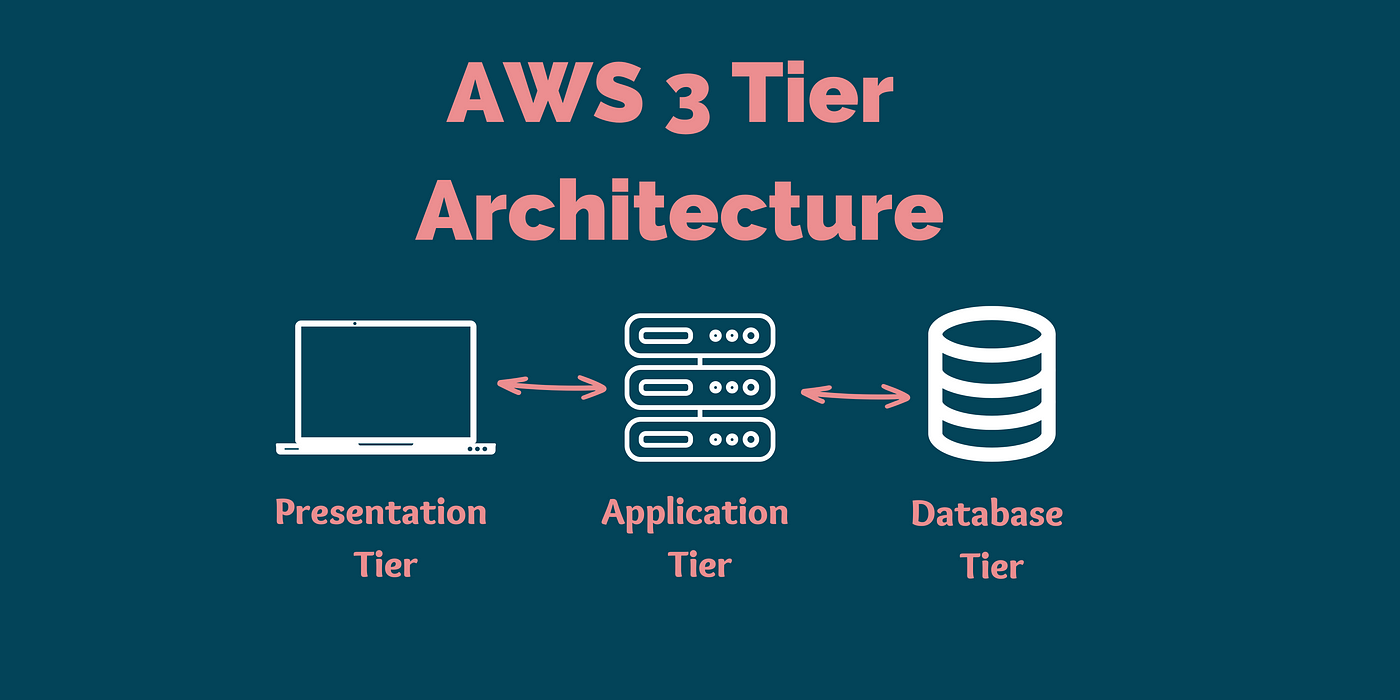
\includegraphics[width=100mm]{slike/arhitektura.png}
		\caption{Arhitektura sustava}
		\label{fig:arhitektura}
	\end{figure}

	\indent{\textit{\underline{Web preglednik}} je program koji korisniku omogućuje pregled
	web-stranica i multimedijalnih sadržaja vezanih uz njih. Svaki web preglednik je predvoditelj korištenja web aplikacija,
	jer omogućuje korisniku da preko web preglednika šalje zahtjeve web poslužitelju.}

	\indent{\textit{\underline{Web poslužitelj}} je osnova rada web aplikacije. On pokreće cijeli sustav rada aplikacije
	te joj prosljeđuje zahtjeve od korisnika. Osnovna zadaća web poslužitelja je omogućiti komunikaciju između korisnika i aplikacije, a ta
	komunikacija se odvija preko HTTP protokola. To je vrsta protokola koja se koristi za prijenos informacija na internetu.}

	\indent{\textit{\underline{Web aplikacija}} je dio web poslužitelja koja služi korisniku za obradu željenih zahtjeva.
	Web aplikacija radi tako da prima zahtjeve i ovisno o zahtjevu pristupa {\textit{\underline{bazi podataka}}} iz koje dohvaća
	"odgovore" na željene zahtjeve. Te "odgovore" šalje natrag korisniku preko web poslužitelja u obliku HTML dokumenta kojeg
	korisnik vidi u web pregledniku.}

	\indent{Programski jezik kojeg smo odabrali za izradu naše web aplikacije je Python. U sklopu Pythona koristimo Django, radni okvir koji služi za izradu web aplikacija. Razvojno okruženje koje koristimo
	je Microsoft Visual Studio Code. Arhitektura sustava temelji se na MVC odnosno MTV konceptu.}

	\indent{Django je modeliran oko MVC arhitekture, no svoju arhitekturu definira kao MTV (eng. {\textit{Model-Template-View}})
	arhitekturu. Komponentu upravitelj (eng. {\textit{Controller}}) zamjenjuje komponentom pogled (eng. {\textit{View}}) te
	komponentu pogled s komponentom predložak (eng. {\textit{Template}}). MTV razdvaja različite dijelove web-stranice: prikaz,
	pristup podatcima i logiku web stranice. Također omogućava neovisnu izgradnju web-stranica, povećava sigurnost sustava te
	pojednostavljuje održavanje sustava.}

	\noindent{MTV se sastoji od:}
	\begin{itemize}
		\item 	\textbf{Model} - definira oblike i odnose podataka u bazi podataka. Model u Django okruženju je klasa napisana
				u programskom jeziku Python. Određuje varijable i metode pridužene određenim tipovima podataka te ima značenje
				tablice u bazi podataka. Model je usko povezan s bazom podataka i pogledom. Od baze podataka model dohvaća tražene
				podatke i prosljeđuje ih pogledu.
		\item 	\textbf{Predložak} - sloj arhitekture MTV-a usko povezan s web-preglednikom. Predložak je HTML stranica s dodanim
				strukturama koje omogućavaju prikaz podataka koji su proslijeđeni od pogleda. Zadaća predloška je sadržaj primljen
				od pogleda organizirati i ugraditi u HTML kod koji će se prikazati u web-pregledniku.
		\item 	\textbf{Pogled} - određuje koji će podatci biti prikazani, odnosno, koji će podatci biti dohvaćeni iz baze podataka
				i prikazani pomoću predloška u web-pregledniku. U Djangu prilikom stvaranja nove web-aplikacije za svaku pojedinu
				aplikaciju stvara se zasebna datoteka pogleda. Pogled ne zna kako su podatci prikazani u web-pregledniku. Posao
				pogleda je dohvatiti tražene podatke i proslijediti ih višem sloju koji će ih prikazati u pregledniku.
	\end{itemize}
	
		

		

				
		\section{Baza podataka}
			
		{Potrebe sustava za bazu podataka su relativno jednostavne, a relacije između entiteta nisu osobito kompleksne. Zbog tih razloga, sustav za bazu podataka koristi MongoDB – \textit{NoSQL}, dokumentno-orijentiranu bazu podataka.} \\ {Entiteti za pohranjivanje podataka su:}
		\begin{itemize}
			\item 	\textbf{Word}{,}
			\item 	\textbf{PronunciationAudio}{,}
			\item 	\textbf{Dictionary}{,}
			\item 	\textbf{Account}{.}
			\item 	\textbf{WordProgress}{,}
			\item 	\textbf{DictionaryProgress}{.}
		\end{itemize}
		{Zvučni zapis izgovora riječi odvojen je od same riječi na koju se odnosi jer je zvučna datoteka relativno veća od ostatka podataka za riječ čime se ubrzava vrijeme dohvata riječi kada se ne koristi način učenja slovkanjem riječi uz dani izgovor.}
		
			\subsection{Opis tablica}
			

				\textit{Važno je istaknuti da je svakom MongoDB dokumentu automatski pridodjeljen , uz ostale atribute, jedinstveni ObjectId u "\_id" atributu (primarni ključ) te je on u tablicama prikazan samo ondje gdje se eksplicitno koristi.} \\
				
				\textbf{Word} \\ {Opisuje riječ. Više rječnika može sadržavati iste riječi pa je veza \textit{N..N}. Sadrži strani ključ na zvučni zapis izgovora riječi na ciljanom jeziku. Veza sa zvučnim zapisom je \textit{N..1}. Svi dokumenti entiteta \textbf{Word} sadržani su u kolekciji "Words".}
				
				\begin{longtblr}[
					label=none,
					entry=none
					]{
						width = \textwidth,
						colspec={|X[8,l]|X[6, l]|X[20, l]|}, 
						rowhead = 1,
					} %definicija širine tablice, širine stupaca, poravnanje i broja redaka naslova tablice
					\hline \SetCell[c=3]{c}{\textbf{Word}}	 \\ \hline[3pt]
					\SetCell{LightGreen}\_id & objectId	&  	Primarni ključ riječi.  	\\ \hline
					word & string	&  	Zapis riječi na ciljanom jeziku.  	\\ \hline
					translation	& string &   Prevedeni zapis riječi na hrvatskom.	\\ \hline 
					descriptionLang & string	&  	Opis riječi na ciljanom jeziku.	\\ \hline
					descriptionCro & string	&  	Opis riječi na hrvatskome jeziku.	\\ \hline  
					\SetCell{LightBlue} audio\_id	& objectId &   Primarni ključ zvučnog zapisa izgovora riječi na ciljanom jeziku.	\\ \hline 
				\end{longtblr}
				
				\textbf{PronunciationAudio} \\ {Sadrži zvučni zapis izgovora na ciljanom jeziku nekih riječi. Veza s riječima je \textit{1..N} u slučaju postojanja homofona. Svi dokumenti entiteta \textbf{PronunciationAudio} sadržani su u kolekciji "PronunciationAudios".}
				
				\begin{longtblr}[
					label=none,
					entry=none
					]{
						width = \textwidth,
						colspec={|X[8,l]|X[6, l]|X[20, l]|}, 
						rowhead = 1,
					} %definicija širine tablice, širine stupaca, poravnanje i broja redaka naslova tablice
					\hline \SetCell[c=3]{c}{\textbf{PronunciationAudio}}	 \\ \hline[3pt]
					\SetCell{LightGreen}\_id & objectId	&  	Primarni ključ zvučnog zapisa.  	\\ \hline
					audio	& binData &   Binarni zapis .mp3 datoteke zvučnog zapisa izgovora na ciljanom jeziku.	\\ \hline 
				\end{longtblr}
				
				\textbf{Dictionary} \\ {Opis rječnika. Riječi riječnika zapisane su kao polje referenci na dokumente entitete \textbf{word} u atributu "words". Veza s riječima je \textit{N..N} jer više rječnika mogu sadržavati istu riječ. Svi dokumenti entiteta \textbf{Dictionary} sadržani su u kolekciji "Dictionaries".}
				
				\begin{longtblr}[
					label=none,
					entry=none
					]{
						width = \textwidth,
						colspec={|X[8,l]|X[6, l]|X[20, l]|}, 
						rowhead = 1,
					} %definicija širine tablice, širine stupaca, poravnanje i broja redaka naslova tablice
					\hline \SetCell[c=3]{c}{\textbf{Dictionary}}	 \\ \hline[3pt]
					\SetCell{LightGreen}\_id & objectId	&  	Primarni ključ rječnika.  	\\ \hline
					name	& string &   Ime rječnika.	\\ \hline 
					language	& string &   Ciljani jezik rječnika.	\\ \hline
					\SetCell{LightBlue} words	& array &   Polje referenci na dokumenate riječi koje čine rječnik.	\\ \hline  
				\end{longtblr}
				
				\textbf{Account} \\ {Opis profila. Administratorske profile od učeničkih profila razlikujemo atributom "isAdmin". Svi dokumenti entiteta \textbf{Account} sadržani su u kolekciji "Accounts".}
				
				\begin{longtblr}[
					label=none,
					entry=none
					]{
						width = \textwidth,
						colspec={|X[8,l]|X[6, l]|X[20, l]|}, 
						rowhead = 1,
					} %definicija širine tablice, širine stupaca, poravnanje i broja redaka naslova tablice
					\hline \SetCell[c=3]{c}{\textbf{Account}}	 \\ \hline[3pt]
					\SetCell{LightGreen}\_id & objectId	&  	Primarni ključ profila.  	\\ \hline
					username	& string &   Korisničko ime profila. (Alternativni primarni ključ)	\\ \hline 
					email	& string &   Adresa e-pošte profila. (Alternativni primarni ključ)	\\ \hline 
					encryptedPass	& string &   SHA-256 kôd lozinke profila.	\\ \hline
					firstName	& string &   Ime vlasnika profila.	\\ \hline 
					lastName	& string &   Prezime vlasnika profila.	\\ \hline 
					isAdmin	& boolean &   Naznaka posjeduje li profil administratorske privilegije.	\\ \hline
					hasInitialPass	& boolean &   Naznaka je li korisnik promijenio inicijalnu lozinku dodijeljenju prilikom registracije. False ... inicijalna lozinka nije promijenjena.     True ... inicijalna lozinka je promijenjena.	\\ \hline  
				\end{longtblr}
				
				\textbf{WordProgress} \\ {Opis napretka učenja određene riječi. Dokumenti entiteta \textbf{WordProgress} pojavljuje se kao ugradbeni dokumenti u dokumentima entiteta \textbf{WordProgress}.}
				
				\begin{longtblr}[
					label=none,
					entry=none
					]{
						width = \textwidth,
						colspec={|X[8,l]|X[6, l]|X[20, l]|}, 
						rowhead = 1,
					} %definicija širine tablice, širine stupaca, poravnanje i broja redaka naslova tablice
					\hline \SetCell[c=3]{c}{\textbf{WordProgress}}	 \\ \hline[3pt]
					\SetCell{LightBlue} word\_id	& objectId &   Referenca na riječ čiji se napredak zabilježava.	\\ \hline 
					timeExpiry	& timestamp &   UNIX vrijeme nakon kojeg je riječ potrebno ponovno ispitati. Vrijeme posljednjeg ispitivanja + vrijeme isteka trenutne posude.	\\ \hline
					currBox	& int &   Trenutna posuda u kojoj se riječ nalazi. Dopuštene vrijednosti: 1, ..., n, n + 1. Ako se riječ nalazi u n + 1. posudi, smatra se naučenom.	\\ \hline
				\end{longtblr}
				
				\textbf{DictionaryProgress} \\ {Opis napretka učenja određenog rječnika od strane određenog učenika.  Svi dokumenti entiteta \textbf{DictionaryProgress} sadržani su u kolekciji "DictionariesProgress".}
				
				\begin{longtblr}[
					label=none,
					entry=none
					]{
						width = \textwidth,
						colspec={|X[8,l]|X[6, l]|X[20, l]|}, 
						rowhead = 1,
					} %definicija širine tablice, širine stupaca, poravnanje i broja redaka naslova tablice
					\hline \SetCell[c=3]{c}{\textbf{DictionaryProgress}}	 \\ \hline[3pt]
					\SetCell{LightBlue} account\_id	& objectId &   Referenca na profil koji uči referencirani rječnik.	\\ \hline 
					\SetCell{LightBlue} dict\_id	& objectId &   Referenca na rječnik kojeg referencirani profil aktivno uči.	\\ \hline
					learningMode	& int &   Trenutni način učenja referenciranog rječnika za referenciranog korisnika. Dopuštene vrijednosti: 1 (prijevod na ciljani jezik), 2 (prijevod na hrvatski), 3 (slovkanje), 4 (izgovor).	\\ \hline
					\SetCell{LightBlue} wordsProgress	& array &   Polje napretka svih riječi referenciranog rječnika, tj. polje ugrađenih dokumenata entiteta \textbf{WordProgress}.	\\ \hline 
				\end{longtblr}
			
			\subsection{Dijagram baze podataka}
			
			\textit{Važno je istaknuti da je svakom MongoDB dokumentu automatski pridodjeljen , uz ostale atribute, jedinstveni ObjectId u "\_id" atributu (primarni ključ) te je on u tablicama prikazan samo ondje gdje se eksplicitno koristi.} \\
				
			\begin{figure}[H]
				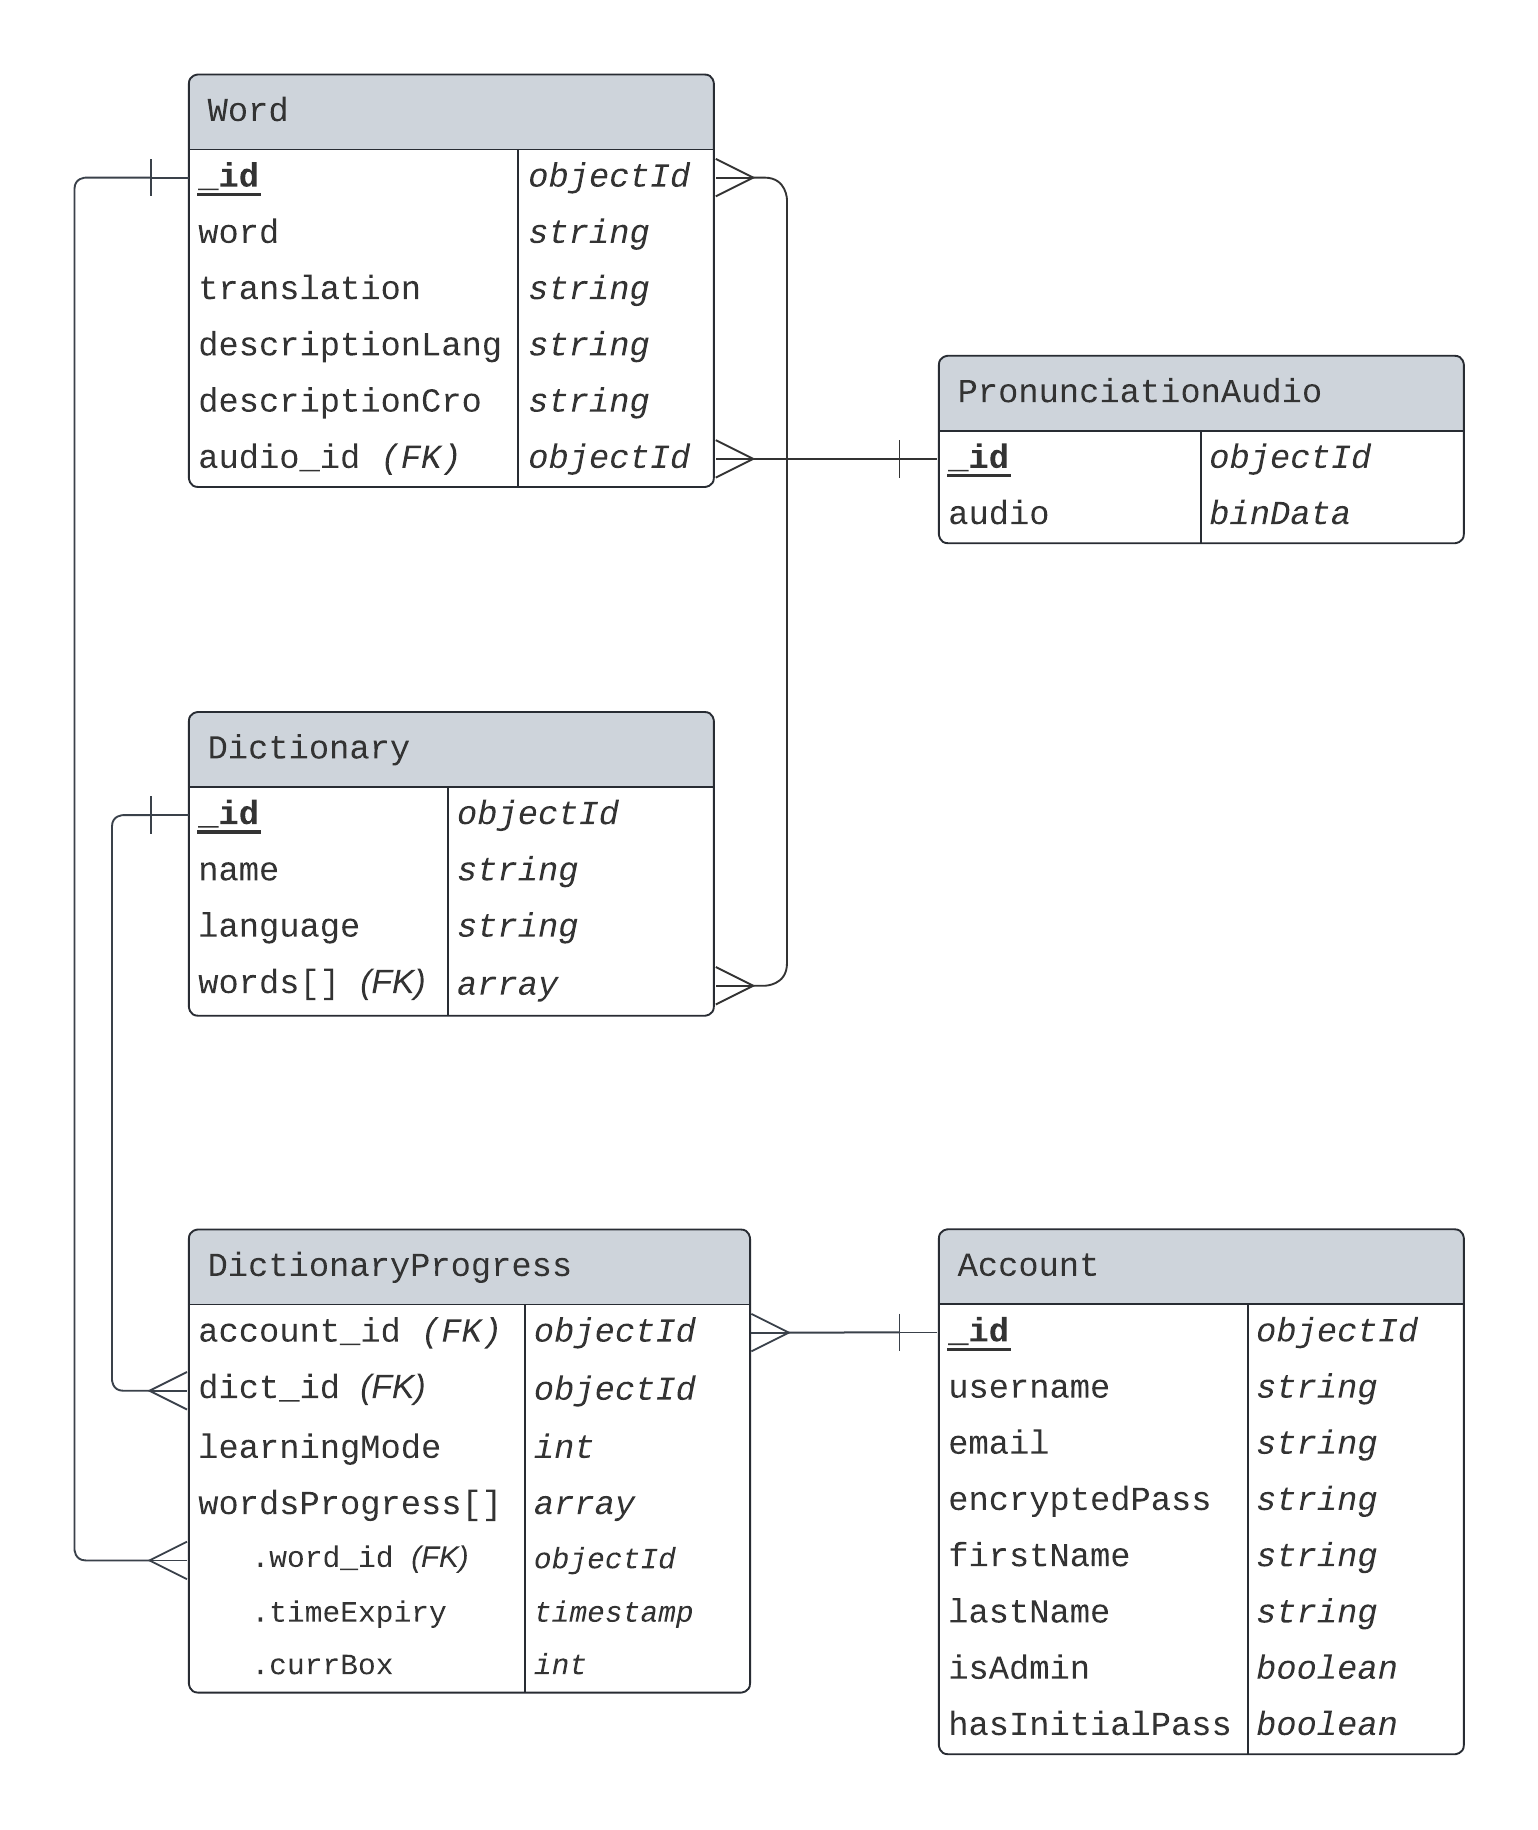
\includegraphics[width=\textwidth]{dijagrami/CanonPrinterDB.png} %veličina u odnosu na širinu linije
				\caption{Dijagram baze podataka}
				\label{fig:ER_dijagram} %label mora biti drugaciji za svaku sliku
			\end{figure}
			
			\eject
			
			
		\section{Dijagram razreda}

			\indent{Na slikama 4.3, 4.4 i 4.5 su prikazani razredi koji pripadaju {\textit{backend}} dijelu MVC (MTV)
			arhitekture. Razredi prikazani na slici 4.3 pirkazuju Controller razred. Metode implementirane u tim razredima
			manipuliraju s DTO razredima ({\textit{Data transfer object}}) koji služe za prijenos podataka između baze podataka i
			aplikacije. Atributi koji se nalaze u DTO razredima dohvaćaju se pomoću metoda implementiranih unutra Model razreda. 
			Metode implementirane unutar Controller razreda vraćaju JSON datoteke.}

			\indent{Zbog lakše oraganizacije, razredi su podijeljeni logički po pravu pristupa metodama određenih aktora. Kako
			bi se smanjila prenatrpanost unutar pojedinog dijagrama, prikazane su samo ovisnosti između razreda koji pripadaju
			istom dijelu dijagrama. Također se iz naziva i tipova atributa može zaključiti vrsta ovisnosti i povezanosti između
			različitih razreda.}

			\begin{figure}[H]
				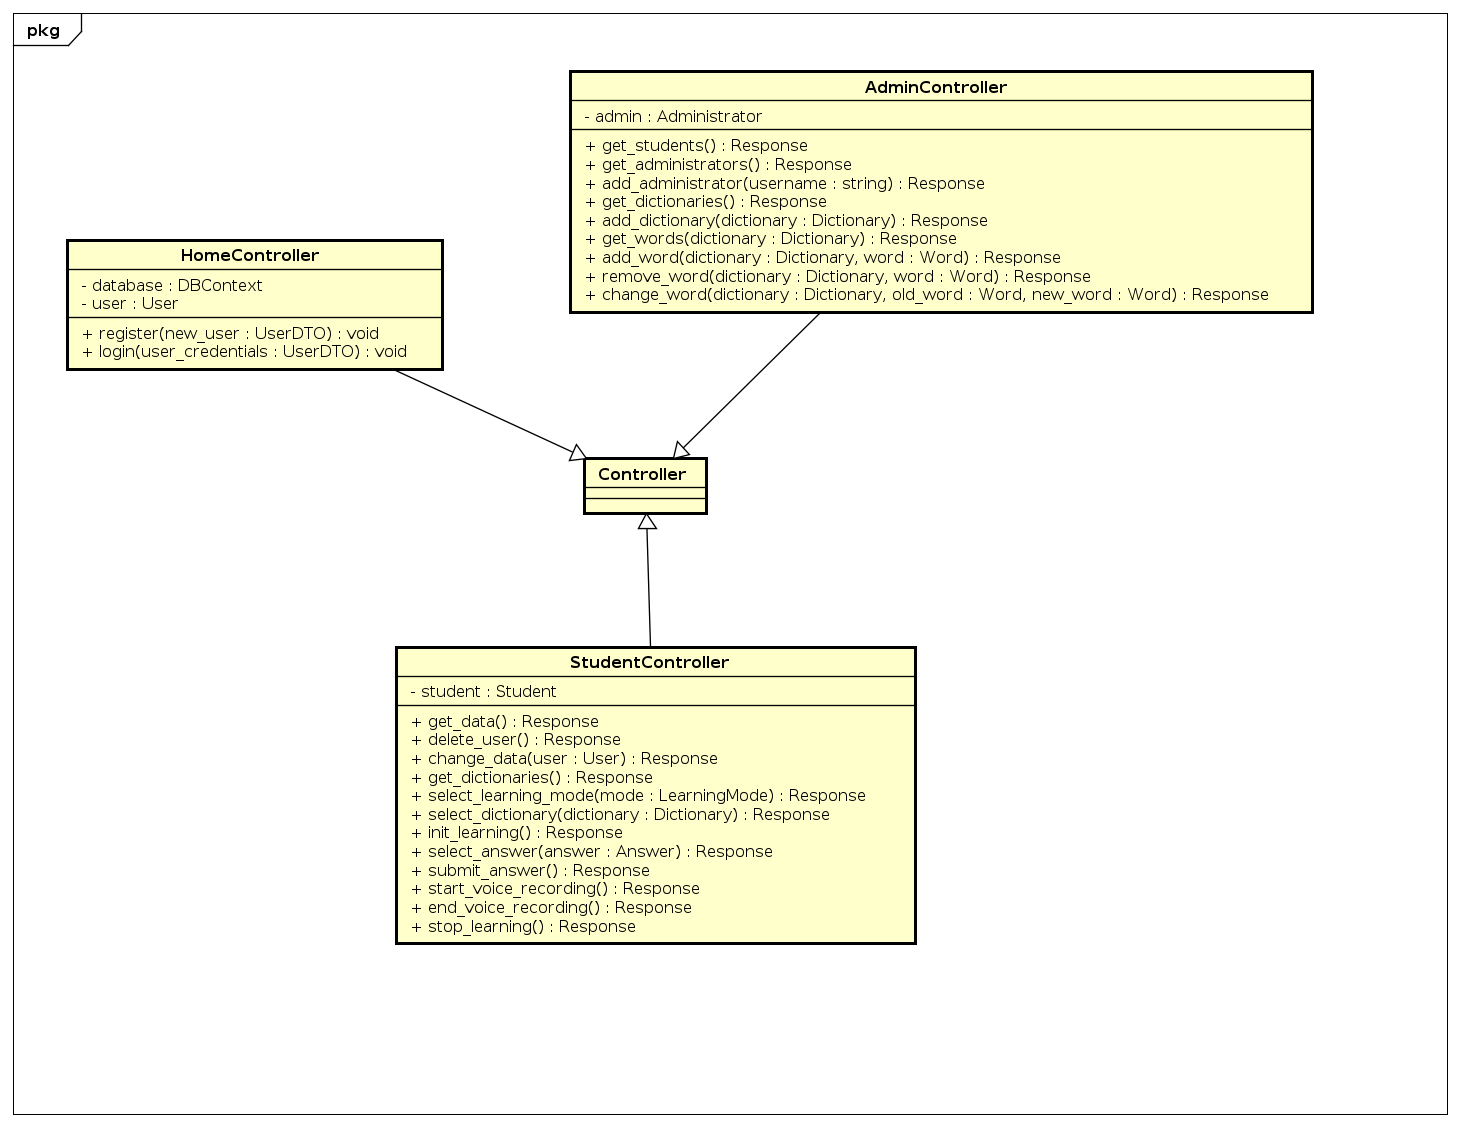
\includegraphics[width=\textwidth]{dijagrami/classcont.png} %veličina u odnosu na širinu linije
				\caption{Dijagram razreda - dio Controllers}
				\label{fig:classcont} %label mora biti drugaciji za svaku sliku
			\end{figure}

			\begin{figure}[H]
				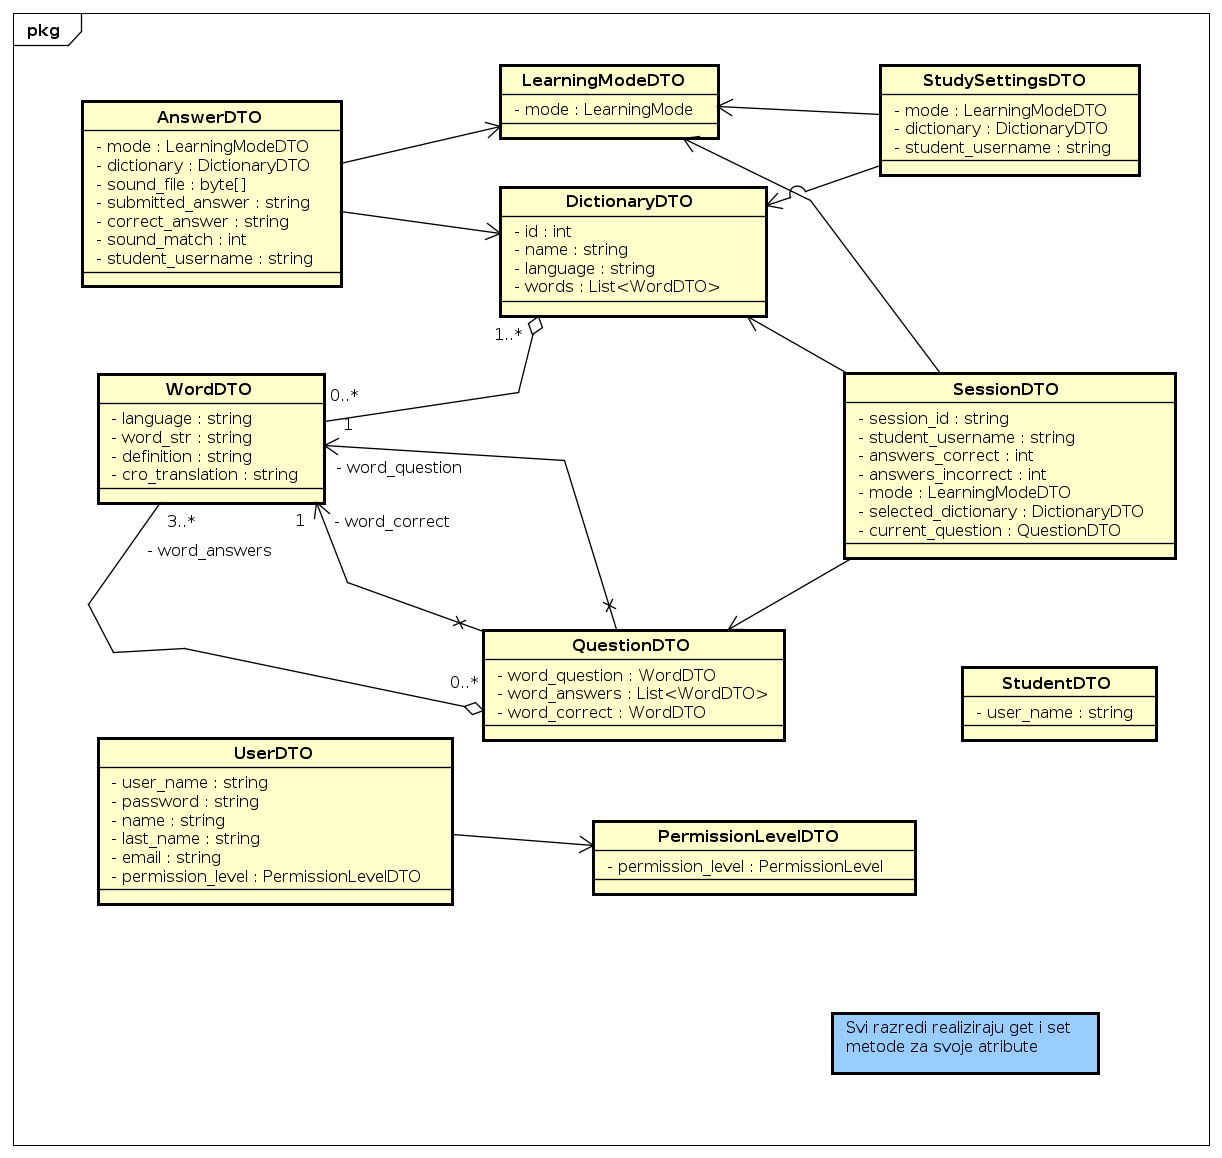
\includegraphics[width=\textwidth]{dijagrami/classdto.png} %veličina u odnosu na širinu linije
				\caption{Dijagram razreda - dio Data Transfer Objects}
				\label{fig:classdto} %label mora biti drugaciji za svaku sliku
			\end{figure}

			\indent{Model razredi zapravo preslikavaju strukturu baze podataka u aplikaciji. Implementirane metode direktno
			komuniciraju s bazom podataka i vraćaju tražene podatke. Razred CustomUser predstavlja korisnika koji se može
			registrirati u aplikaciju (ako nema već kreiran korisnički račun), ulogirati u aplikaciju, pregledavati i mijenjati
			svoje korisničke podatke te izbrisati svoj korisnički račun. Na razred CustomUser se vežu razredi Administrator i
			Student koji predstavljaju korisnike aplikacije. Razred CustomUser je također povezan s razredom PermissionLevel
			u kojem je zapisano koju razinu dozvole ima korisnik te se prema tome određuje je li korisnik Student ili Administrator.
			Razred Administrator je povezan s razredima Dictionary i Word jer administrator ima mogućnost uređivanja rječnika
			u aplikaciji. Razred Student je povezan s razredima Dictionary (student može odabrati rječnik za učenje), LearningMode
			(student odabire način učenja jezika) i s razredom Session. Razred Session predstavlja srž aplikacije, što je učenje
			stranog jezika. Povezan je s razredima Answer, Question i LearningMode, a preko tih razreda i s razredima Dictionary,
			Word itd. Taj razred služi za pohranu studentovog odgovora, pitanja, izgovora riječi, načina učenja... te u njemu
			student prekida svoje učenje.}

			\begin{figure}[H]
				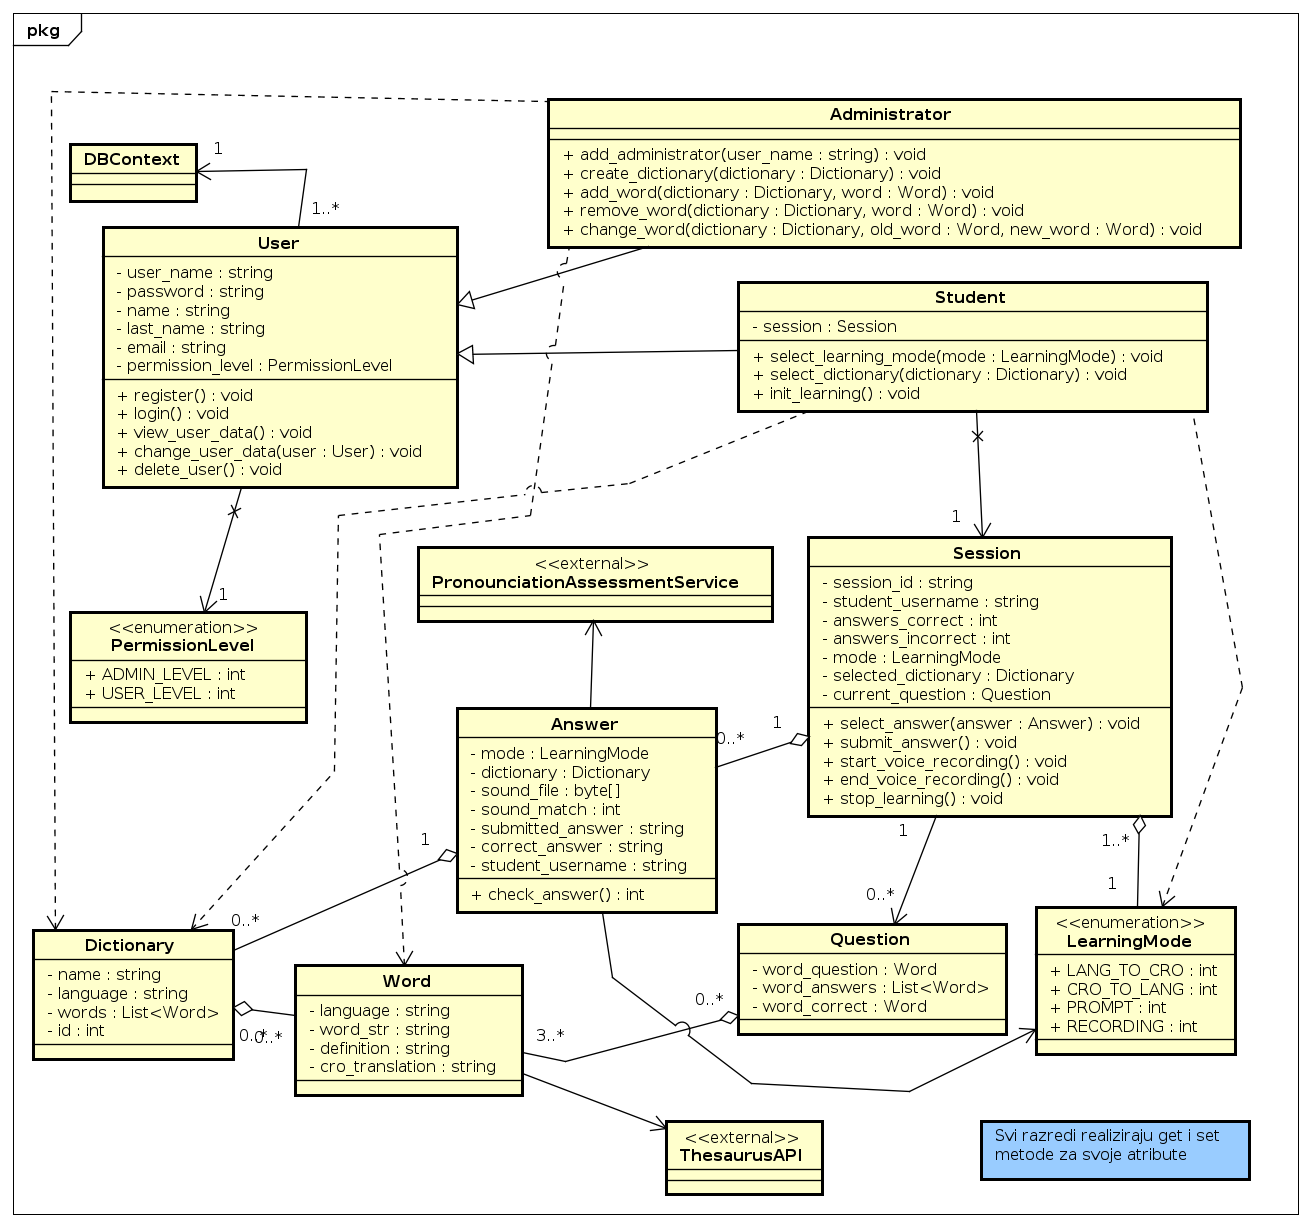
\includegraphics[width=\textwidth]{dijagrami/classmodel.png} %veličina u odnosu na širinu linije
				\caption{Dijagram razreda - dio Models}
				\label{fig:classmodel} %label mora biti drugaciji za svaku sliku
			\end{figure}
					
			
			\eject
		
		\section{Dijagram stanja}
			
			\noindent{Slika \ref{fig:Dijagram stanja učenika} prikazuje stanja kroz koje se može naći učenik koristeći aplikaciju.} \\
			\indent{Svakom korisniku prilikom posjeta aplikaciji se prikazuje uvodna stranica gdje se korisnik može, ukoliko već posjeduje račun, prijaviti pritiskom na tipku "Login" u gornjem desnom kutku prilikom čega će se od korisnika tražiti adresa e-pošte i lozinka. Nakon unosa te pritiskom na tiku Log in ispod unosa, ukoliko su vjerodajnice ispravne, korisnik će biti prijavljen. Ako korisnik ne posjeduje račun, moguće ga je registrati pritiskom na tipku "Sign up" u gornjem desnom kutku prilikom čega se od korisnika zahtjeva da upiše svoju adresu e-pošte na koju će se poslati inicijalna lozinka. Nakon unosa adrese e-pošte te pritiskom na tipku "Sign up" ispod unosa, korisnika se vraća na uvodnu stranicu gdje se može prijaviti s inicijalnom lozinkom dobivenu na adresu e-pošte. Nakon prve prijave od registracije, od korisnika se zahtjeva promjena inicijalne lozinke. Ovaj korak nije moguće zaobići i od korisnika će se zahtjevati promjena inicijalne lozinke prilikom svake prijave dok ju ne promijeni. } \\			\indent{Kada se učenik uspješno prijavi u sustav, prikazuje mu se učenička stranica na kojoj može nastaviti učiti rječnike, pregledavati sve rječnike, ažurirati podatke računa i odjaviti se. Dodantno, nakon svake prijave se u web-preglednik zapisiju kolačići vezani za prijavu tako da kada korisnik ponovno posjeti aplikaciju u istom web-pregledniku, biti će automatski prijavljen.} \\
			\indent{Da bi učenik započeo, ili nastavio, učenje nekog rječnika, potrebno ga je odabrati pritiskom na tipku "Customize learning" prilikom čega će se ponuditi opcija odabira jezika, a nakon odabira jezika ponudit će se svi rječnici na odabranom jeziku. Odabirom jednog od ponuđenih rječnika potrebno je još i odabrati načine učenja. Dostupna su 4 načina učenja: (1) upitom riječi iz rječnika uz odabir hrvatskog prijevoda: (2) upitom hrvatske riječi uz odabir prijevoda na jezik rječnika; (3) izgovorom riječi iz rječnika uz slovkanje riječi; (4) upitom riječi iz rječnika uz snimanje izgovora riječi. Svi načini učenja sastoje se od niza pitanja gdje se od učenika zahtjeva odabri točnog odgovora, točan izgovor ili točno slovkanje. Učenje se prekida pritiskom na tipku "FINISH" prilikom čega se učenika vraća na učeničku stranicu. } \\
			\indent{Na učeničkoj stranici moguće je i pregledati sve rječnike pritiskom na tipku "View dictionary" prilikom čega se od učenika traži jezik rječnika, a tek onda odabir rječnika na odabranom jeziku. Prikazati će se samo riječi iz rječinka bez prijevoda ili mogućnosti slušanja izgovora.} \\
			\indent{Učenik je u mogućnositi u svakom trenutku pregledati podatke svojeg računa i upravljati računom pritiskom na tipku "Profile" u gornjem  desnom kutku prilikom čega se učeniku prikazuje stranica za pregled i upravljanje računom. Ukoliko učenik želi promijeniti neki podatak, klikom na odgovrajuće polje može unijeti ažurirani podatak. Učenik može više podataka promijeniti odjednom, a svi promijenjeni podaci se ažuriraju tek nakon pritiska tipke "Save Changes". Važno je napomenuti da adresu e-pošte nije moguće promijeniti. Ukoliko učenik želi izbrisati račun, potrebno je pritisnuti tipku "Delete Account". Također je u svakom trenutku moguće odjaviti se čime se korisnika vraća na uvodnu stranica aplikacije, a kolačići za prijavu brišu tako da prilikom sljedećeg posjeta aplikaciji ne bude automatski prijavljen.}
			
			\begin{figure}[H]
				\centering
				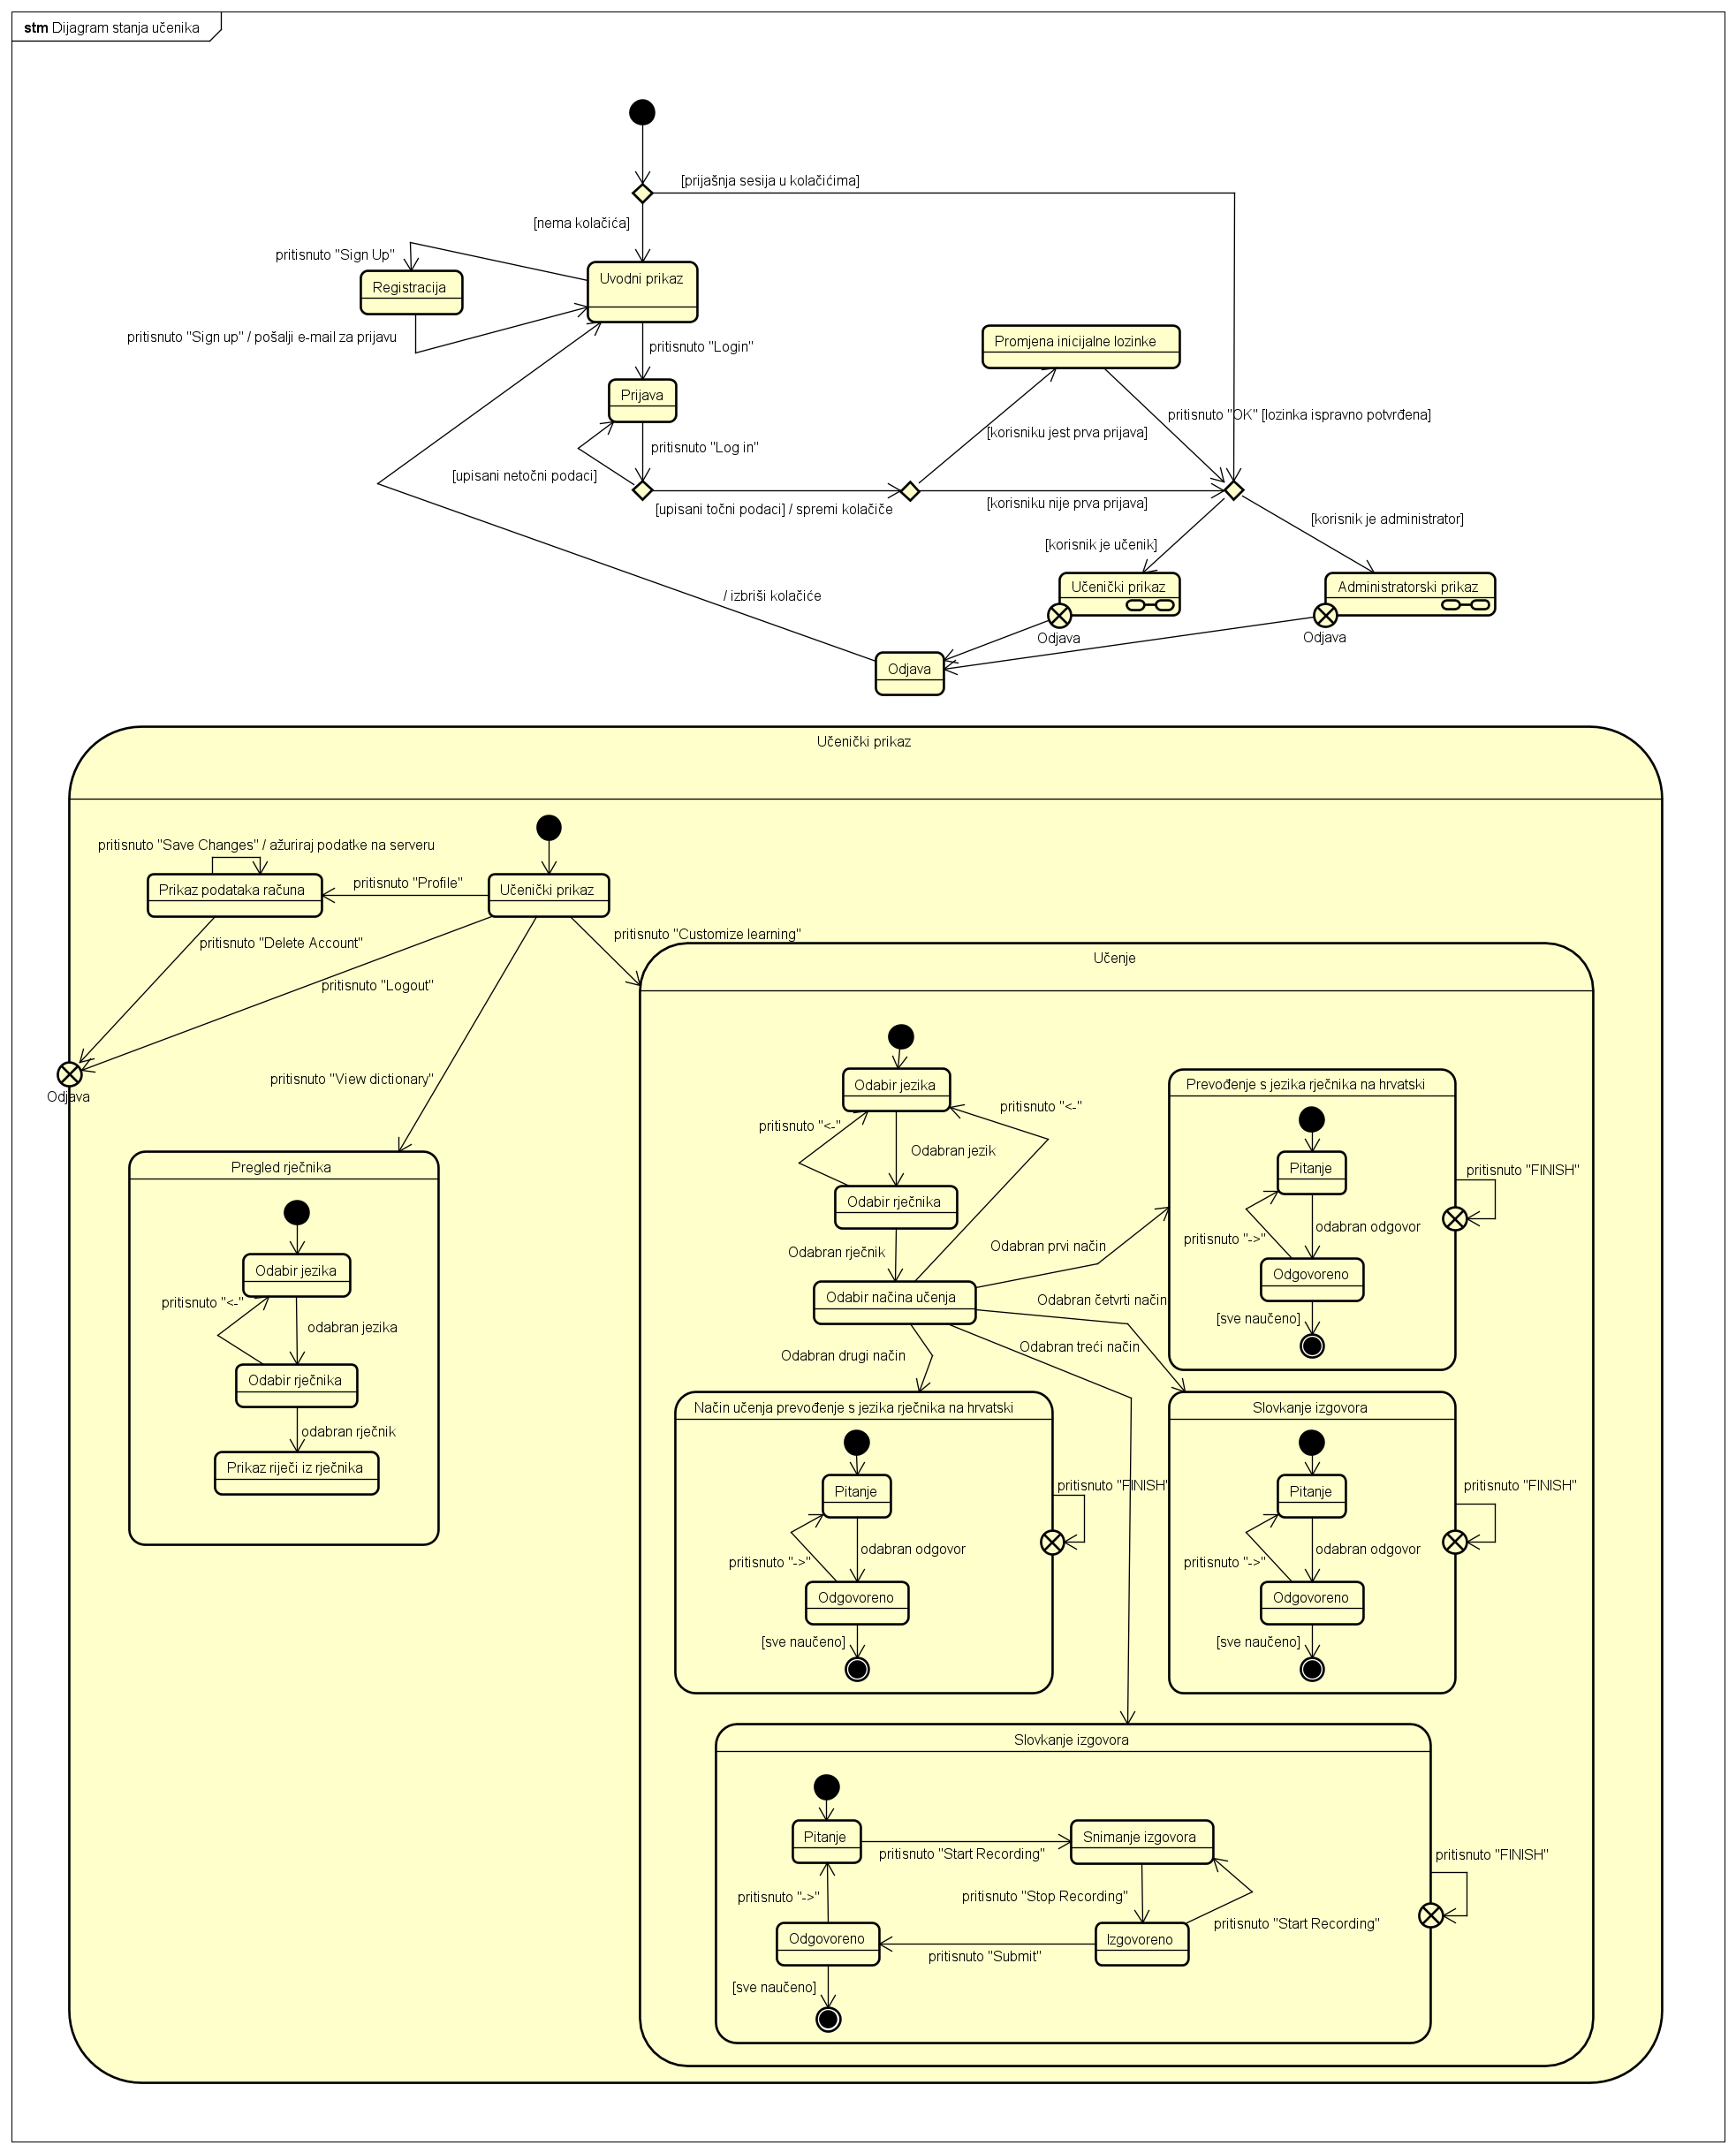
\includegraphics[width=\textwidth]{dijagrami/Dijagram_stanja_ucenika.png}
				\caption{Dijagram stanja učenika}
				\label{fig:Dijagram stanja učenika}
			\end{figure}
			
			
			\eject 
		
		\section{Dijagram aktivnosti}
		
			\noindent{Slika \ref{fig:Dijagram aktivnosti dodavanja nove riječi} prikazuje dijagram aktivnosti sustava kada administrator dodaje novu riječ.} \\
			\indent{Za dodavanje nove riječi administrator je dužan unjeti podatke o novoj riječi, a to su: vrsta riječi, sama riječ, opis riječi na jeziku rječnika, prijevod na hrvatski i riječnik kojem će riječ pripadati. Prilikom tipkanja same riječi, web-aplikacija će na svaku promjenu upisa regairati tako da predloži nekolicinu riječi na osnovi teksta koje je administrator do tada utipkao. Administrator tada može odabrati svoju riječ ako se nalazi u listi prijedloga, a ako ne, natipkati ju do kraja. Dodatno, kada administrator upiše riječ, web-aplikacija će automatski popuniti polje za opis riječi prikladnim opisom za tu riječ na osnovi vrste riječi. Administrator opis po volji može mijenjati.} \\
			\indent{Kada je administrator upisao sve potrebne podatke o novoj riječi, može pritisnuti gumb "Add word" prilikom čega će web-aplikacija slati zahtjev na server za dodaju nove riječi. Prije dodaje riječi, server u svojoj bazi podataka provjerava je li ista riječ već postoji u zadanom rječniku, ako postoji, ignorirat će zahtjev, a ako riječ ne postoji u rječniku, onda će ju uspješno dodati.}

			\begin{figure}[H]
				\centering
				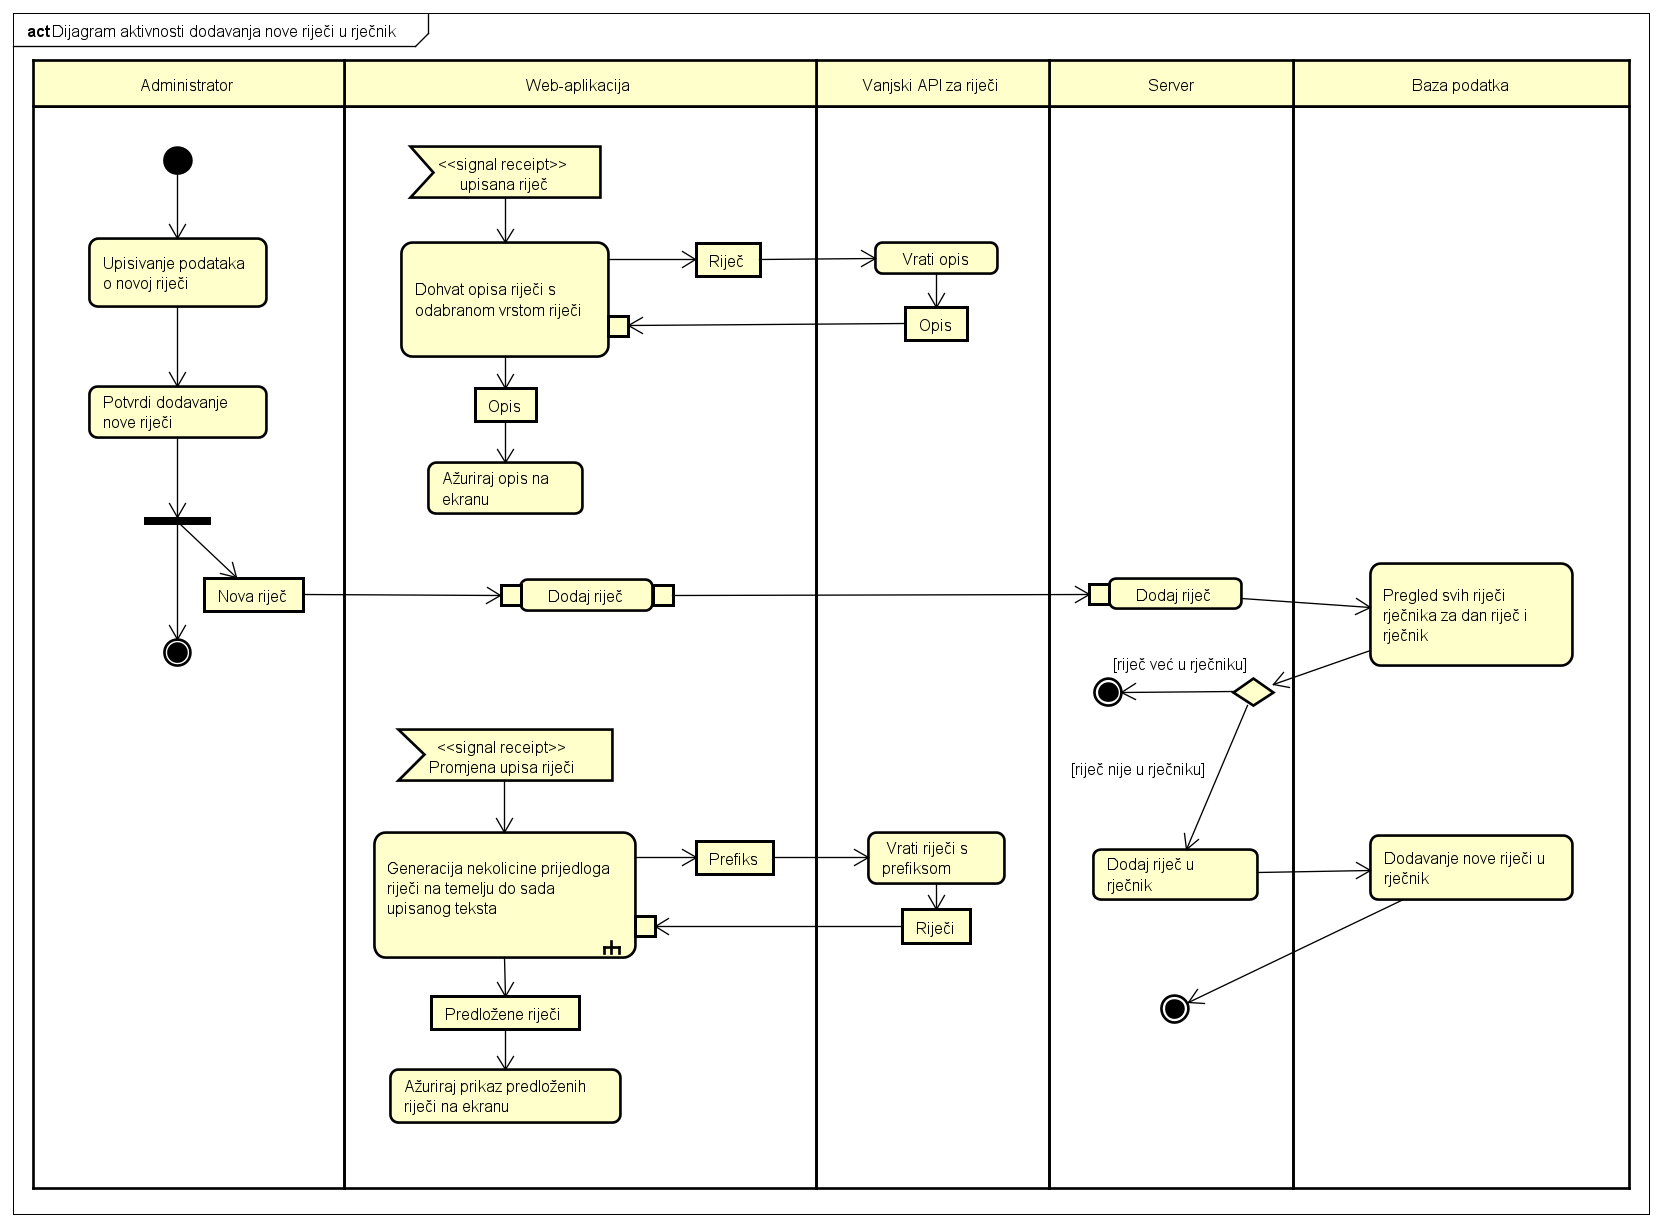
\includegraphics[width=\textwidth]{dijagrami/Dijagram_aktivnosti_dodavanja_nove_rijeci.png}
				\caption{Dijagram aktivnosti dodavanja nove riječi}
				\label{fig:Dijagram aktivnosti dodavanja nove riječi}
			\end{figure}
			
			\eject
		\section{Dijagram komponenti}
		
			\textbf{\textit{dio 2. revizije}}\\
		
			 \textit{Potrebno je priložiti dijagram komponenti s pripadajućim opisom. Dijagram komponenti treba prikazivati strukturu cijele aplikacije.}